\subsection{MIR Initializer Expressions}

\begin{figure}
  \centering
  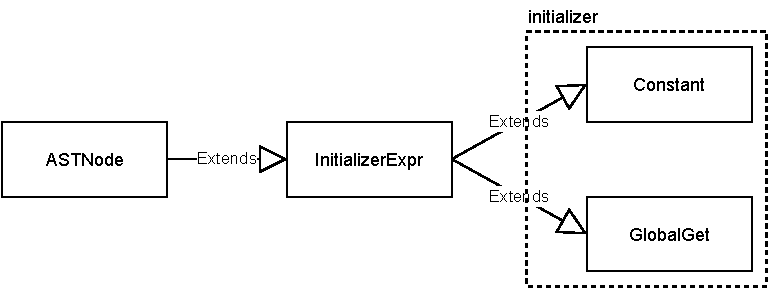
\includegraphics[width=\textwidth]{Images/4.MIR/initializer-expression.pdf}
  \caption{SableWasm MIR Initializer Expression}
  \label{fig:sablewasm-mir-initializer-expression}
\end{figure}

WebAssembly defines a particular form of expression, namely constant expressions. They can appear in three locations in the current specification. First, global variables declaration can contain constant expression as their initialization values. Additionally, data section entries and element section entries can have constant expressions as the offsets for their initialization payload. In SableWasm MIR, we define initializer expressions that act similar to what constant expression does in WebAssembly. Figure~\ref{fig:sablewasm-mir-initializer-expression} gives a general illustration about SableWasm MIR initializer expressions. The initializer expressions are quite simple. In the current WebAssembly and SableWasm, an initializer expression can be either a constant value or refer to an imported global via \texttt{GlobalGet} instruction. Hence, in principle, currently, SableWasm MIR initializer expression is essentially a single instruction. In the future, one may generalize such constrain by allowing more complex constructs in initializer expressions. 

\paragraph{Constant}
The \texttt{Constant} instruction represents a single constant value for the initializer expression. In WebAssembly, a constant value can be one of the following: a 32-bit or 64-bit integer, a floating-pointer number or a 128-bit SIMD vector \footnote{with WebAssembly SIMD128 extension}, and the specification encodes type within the instruction opcode. Hence, there are multiple instructions in WebAssembly to introduce a constant. In SableWasm, we do not encode the type into the opcode, and \texttt{Constant} instruction is the only instruction that takes care of the task. In figure~\ref{fig:sablewasm-mir-initializer-expression}, we have a constant initializer at line 6 that initializes the values of the global to a 32-bit integer with a value that equals 66560. When querying the type of a \texttt{Constant} instruction, SableWasm will infer it from its payload constant.

\paragraph{GlobalGet}
The \texttt{GlobalGet} instruction is exactly same as the WebAssembly's \texttt{global.get} in execution semantics. WebAssembly specification allows any initializer refers to an imported \footnote{This might subject to change in the future version of WebAssembly} global value. As these values are initialized before the module, reading the value from them is always valid during module initialization. The example in the figure does not provide an example of \texttt{GlobalGet} as an initializer expression. They are less frequently used compare to constant initializer expression, especially for global values. However, in some ABI implementations, data section entries and element section entries require to read from global values serving as base pointers. SableWasm also infer the type for \texttt{GlobalGet} initializer expression in a similar fashion as \texttt{Constant}. In this case, the type of instruction is the same as the referred global variable without the constness modifier.

In this section, we cover the design and implementation of initializer expressions in SableWasm. They are pretty simple in the current design. We will now move to the next part in the SableWasm design, the module-level entities.